%!TEX program = xelatex
\documentclass[aspectratio=169, 10pt]{beamer}
\usepackage{ifpdf}
\usepackage[active,tightpage]{preview}

\usepackage{tikz}
\usetikzlibrary{arrows.meta, backgrounds, fit, positioning, shapes.geometric, calc, decorations.pathreplacing, decorations.markings,shadows.blur, decorations.pathmorphing}
\PreviewEnvironment{tikzpicture}

\usepackage{xltxtra}
\usepackage{xunicode}

% Fonts
\usepackage{fontspec}
\defaultfontfeatures{Mapping=tex-text}

\usepackage{newtxsf}
\setmainfont{Fira Sans}
\usepackage{mathastext}

\usepackage{hyperref}

\hypersetup{
    colorlinks=true,
    linkcolor=blue,
    urlcolor=blue,
    citecolor=green,
    filecolor=magenta
}

\begin{document}

\tikzset{basic/.style={draw,fill=blue!20,text width=1.5em,text badly centered}}
\tikzset{input/.style={basic,circle}}
\tikzset{weights/.style={basic,rectangle, rounded corners=2pt}}
\tikzset{functions/.style={basic,circle,fill=blue!10}}

\begin{tikzpicture}[>=latex]
    \node[functions] (center) {};
    \node[below of=center,font=\footnotesize,text width=5em] {Activation function};
    \draw[thick] (0.5em,0.5em) -- (0,0.5em) -- (0,-0.5em) -- (-0.5em,-0.5em);
    \draw (0em,0.75em) -- (0em,-0.75em);
    \draw (0.75em,0em) -- (-0.75em,0em);
    \node[right of=center] (right) {};
    \path[draw,->] (center) -- (right);
    \node[functions,left=3em of center] (left) {$\sum$};
    \path[draw,->] (left) -- (center);
    \node[weights,left=3em of left] (2) {$w_2$} -- (2) node[input,left of=2] (l2) {$x_2$};
    \path[draw,->] (l2) -- (2);
    \path[draw,->] (2) to [out=0,in=180] (left);
    \node[below of=2] (dots) {$\vdots$} -- (dots) node[left of=dots] (ldots) {$\vdots$};
    \node[weights,below of=dots] (n) {$w_n$} -- (n) node[input,left of=n] (ln) {$x_n$};
    \path[draw,->] (ln) -- (n);
    \path[draw,->] (n) to [out=0,in=270] (left);
    \node[weights,above of=2] (1) {$w_1$} -- (1) node[input,left of=1] (l1) {$x_1$};
    \path[draw,->] (l1) -- (1);
    \path[draw,->] (1) to [out=0,in=135] (left);
    \node[weights,above of=1] (0) {$w_0$} -- (0) node[input,left of=0] (l0) {$1$};
    \path[draw,->] (l0) -- (0);
    \path[draw,->] (0) to [out=0,in=90] (left);
    \node[below of=ln,font=\footnotesize] {Inputs};
    \node[below of=n,font=\footnotesize] {Weights};

    \node at (4,0) {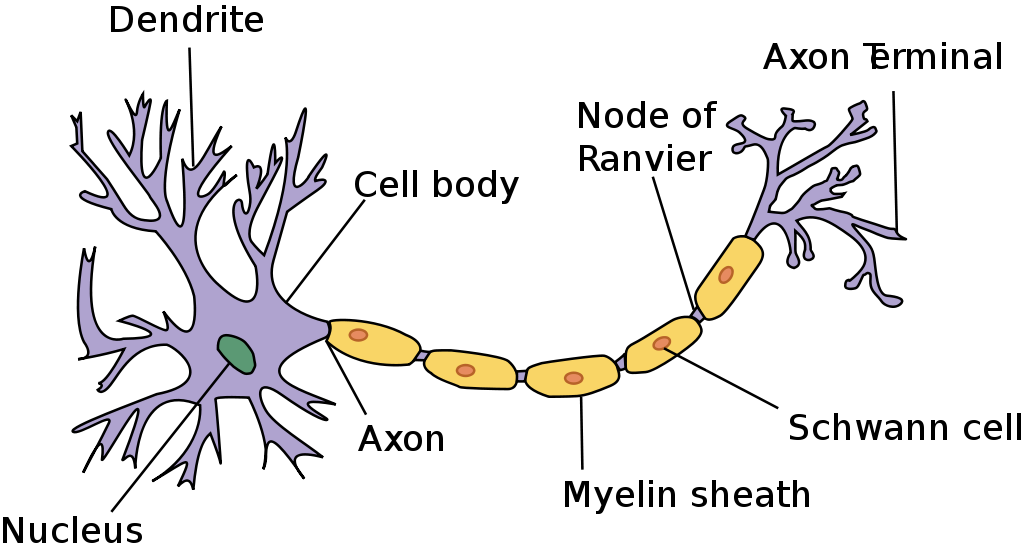
\includegraphics[width=.5\textwidth]{bio-neuron.png}};

    \node[fill=yellow] at (-3,3) {Artificial neuron};
    \node[fill=yellow] at (4,3) {Biological neuron};

\end{tikzpicture}


\end{document}
